\documentclass[multi=tikzpicture,border=7pt]{standalone}
\usepackage{ctex,amsmath,amssymb,bm}
\usepackage{tikz,pgfplots}
\pgfplotsset{compat=1.18}
\usetikzlibrary{arrows.meta,calc,angles,quotes,patterns,positioning,decorations.pathmorphing,3d,intersections}
\tikzset{wire/.style={brown!70!black,very thick},guide/.style={dashed,gray!60},force/.style={->,>=Stealth,thick,red!70!black},velocity/.style={->,>=Stealth,thick,blue!70!black},axis/.style={->,>=Stealth,thick},dim/.style={<->,>=Stealth,thin},body/.style={draw,thick,fill=blue!7},panel/.style={anchor=west,font=\bfseries},hidden/.style={dashed,gray!58,thick},orbit/.style={very thick,blue!70!black}}
\tikzset{charge/.style={circle,draw,fill=blue!12,minimum size=5.5mm,inner sep=0pt},resistor/.style={decorate,decoration={zigzag,segment length=4pt,amplitude=2pt},thick}}
\tikzset{vec/.style={->,>=Stealth,very thick},wall/.style={pattern=north east lines,pattern color=gray},nodept/.style={circle,fill=white,draw,inner sep=1.5pt}}
\tikzset{flow/.style={->,>=Stealth,very thick,blue!70!black},current/.style={->,>=Stealth,very thick,red!70!black},terminal/.style={circle,draw,fill=white,inner sep=1.5pt}}
\begin{document}
% 1 question-01
\begin{tikzpicture}[x=1cm,y=1cm,font=\small]

\draw[very thick] (0,0) circle (2.45);
  \draw[guide] (-3.3,0)--(3.3,0) (0,-3.3)--(0,3.3);
  \draw[dim] (0,0)--(2.45,0) node[midway,above] {$R$};
  \begin{scope}[shift={(0,2.45)},rotate=-12]
    \draw[body,rounded corners=3pt] (-1.1,-.48) rectangle (1.1,.48);
    \draw[thick] (-.72,-.68) circle (.2) (.72,-.68) circle (.2);
    \draw[force] (0,0)--(1.65,0) node[right] {$a$};
    \draw[force] (0,0)--(.35,-1.55) node[right] {$v^2/R$};
  \end{scope}
  \node at (0,-3.0) {后轮驱动汽车在水平圆轨道上加速};

\end{tikzpicture}

% 2 solution-01
\begin{tikzpicture}[x=1cm,y=1cm,font=\small]

\begin{scope}[shift={(-3.3,0)}]\draw[guide](0,0)circle(1.9);\draw[velocity](0,0)--(1.3,0)node[right]{$ma$};\draw[force](1.3,0)--(1.3,1.2)node[above]{$mv^2/(2R)$};\draw[thick](0,0)--(1.3,1.2);\node[align=center]at(0,-2.7){驱动后轮摩擦圆\\$\sqrt{(ma)^2+[mv^2/(2R)]^2}\le\mu mg/2$\\横向等分另需忽略偏航惯性};\end{scope}
\begin{scope}[shift={(3.1,0)}]\draw[axis](0,0)--(0,2)node[above]{$\bm\Omega\parallel\bm e_z$};\draw[velocity](0,0)--(2,0)node[right]{$\bm L\parallel-\bm e_y$};\node[draw,circle]at(0,-1){$\otimes$};\node[right]at(.5,-1){车身 $\bm\tau=-\bm\Omega\times\bm L$};\node[align=center]at(1,-2.7){沿车头看截面，$\bm e_x$ 朝读者\\车轮受 $+\bm e_x$ 力矩，车身受反向力矩};\end{scope}

\end{tikzpicture}

% 3 question-02
\begin{tikzpicture}[x=1cm,y=1cm,font=\small]

\draw[thick](-3,2.5)--(-1.3,.4);\draw[thick](1.3,.4)--(3,2.5);
\draw[orbit](-1.3,.4)..controls(-.45,.35)and(.45,.35)..(1.3,.4);
\draw[guide](0,.36)--(0,3.4);\draw[guide](-1.3,.4)--(-1.35,3.3) (1.3,.4)--(1.35,3.3);
\fill[orange](-2.8,2.25)circle(.12)node[left]{$m$};\draw[dim](-3.5,.4)--(-3.5,2.5)node[midway,left]{$h$};
\node[align=left,anchor=west]at(3.7,1.5){斜面 $\alpha=\pi/4$\\圆弧半角 $\theta=0.01$\\$\rho=10\,\mathrm m$\\两段不相切，原几何示意\\不能直接当连续光滑轨道};

\end{tikzpicture}

% 4 solution-02
\begin{tikzpicture}[x=1cm,y=1cm,font=\small]

\begin{scope}[shift={(-3.3,0)}]\draw[thick](-1.5,2)--(1.5,-1);\fill(0,.5)circle(2pt);\draw[force](0,.5)--(.8,1.3)node[right]{$N$};\draw[force](0,.5)--(0,-.8)node[below]{$mg$};\draw[velocity](0,.5)--(.8,-.3)node[right]{$u$};\node[align=center]at(0,-2){斜面局部有效质量\\$m_s=m(M+m\cos^2\alpha)/(M+m)$};\end{scope}
\begin{scope}[shift={(2.2,0)}]\draw[axis](-2,0)--(2.5,0)node[right]{$x$};\draw[orbit,domain=-1.7:1.7,samples=60]plot(\x,{.5*(\x)^2});\fill[orange](.8,.32)circle(.12);\draw[force](.8,.32)--(.8,-.8)node[right]{$mg$};\node[above]at(.8,.6){$x\simeq\rho\varphi$};\node[align=center]at(0,-2){圆弧局部有效质量\\$m_c=mM/(M+m)$};\end{scope}
\node[align=center]at(0,-3.3){两个局部模型；过渡另需规则\\无损短过渡：$m_su_1^2=m_cu_c^2$；进入圆弧使用 $u_c$};

\end{tikzpicture}

% 5 question-03
\begin{tikzpicture}[x=1cm,y=1cm,font=\small]

\draw[very thick] (-4.7,3.0)--(4.7,3.0);
  \draw[very thick] (-3.8,3)--(-3.8,1.2) node[midway,left] {轻杆};
  \draw[very thick] (3.8,3)--(3.8,1.2) node[midway,right] {待剪细绳};
  \draw[body] (-3.8,1.05) rectangle (3.8,1.35); \node[left] at (-3.8,1.2) {$A$}; \node[right] at (3.8,1.2) {$B$};
  \draw[very thick] (-3.8,1.05)--(-3.8,-1.0) node[midway,left] {$AC$（绳）};
  \draw[very thick] (3.8,1.05)--(3.8,-1.0) node[midway,right] {$BD$（杆）};
  \draw[body] (-3.8,-1.15) rectangle (3.8,-.85); \node[left] at (-3.8,-1.0) {$C$}; \node[right] at (3.8,-1.0) {$D$};
  \draw[force] (-3.8+2.0,1.05)--(-3.8+2.0,-.35) node[right] {$mg$};
  \draw[force] (-3.8+2.7,-1.15)--(-3.8+2.7,-2.55) node[right] {$mg$};
  \draw[dim] (-3.8,.55)--(-1.8,.55) node[midway,below] {$l_1$};
  \draw[dim] (-3.8,-1.75)--(-1.1,-1.75) node[midway,below] {$l_2$};

\end{tikzpicture}

% 6 solution-03
\begin{tikzpicture}[x=1cm,y=1cm,font=\small]

\begin{scope}[shift={(-3.8,0)}]
    \draw[body] (-2.4,.5) rectangle (2.4,.78); \node[left] at (-2.4,.64) {$A$}; \node[right] at (2.4,.64) {$B$};
    \draw[force] (-2.4,.64)--(-2.4,2.0) node[above] {$A_y$};
    \draw[force] (2.4,.64)--(2.4,-1.0) node[below] {$T$};
    \draw[force] (-2.4+1.25,.5)--(-1.15,-1.1) node[below] {$mg$};
    \draw[current] (-1.2,1.6) arc (140:20:1.0) node[right] {$\alpha_1$};
    \node at (0,-1.65) {$m(a^2+l_1^2)\alpha_1=mg l_1+Tl$};
  \end{scope}
  \begin{scope}[shift={(3.8,0)}]
    \draw[body] (-2.4,.5) rectangle (2.4,.78); \node[left] at (-2.4,.64) {$C$}; \node[right] at (2.4,.64) {$D$};
    \draw[force] (2.4,.64)--(2.4,2.0) node[above] {$T$};
    \draw[force] (-2.4+1.7,.5)--(-.7,-1.1) node[below] {$mg$};
    \draw[current] (-1.2,1.6) arc (140:20:1.0) node[right] {$\alpha_2$};
    \node at (0,-1.65) {约束：$a_{D,y}=a_{B,y}$};
  \end{scope}

\end{tikzpicture}

% 7 question-04
\begin{tikzpicture}[x=1cm,y=1cm,font=\small]
\draw[axis](-4,0)--(6,0)node[right]{光轴};\draw[very thick,<->](0,-1.4)--(0,1.4);\draw[very thick,>-<](4,-1.4)--(4,1.4);\fill(-3.07037,0)circle(2pt)node[below]{$O$};\draw[dim](-3.07037,-.9)--(0,-.9)node[midway,below]{$u$};\draw[dim](0,1.7)--(4,1.7)node[midway,above]{$D=2f$};\node[below]at(0,-1.5){$L_1,f$};\node[below]at(4,-1.5){$L_2,-2f$};\draw[very thick](-.66667,-1.2)--(-.66667,-.5) (-.66667,.5)--(-.66667,1.2);\node[above]at(-.66667,.85){光阑};
\end{tikzpicture}

% 8 solution-04
\begin{tikzpicture}[x=1cm,y=1cm,font=\small]
\draw[axis](-4,0)--(8,0);\draw[very thick,<->](0,-1.4)--(0,1.4);\draw[very thick,>-<](4,-1.4)--(4,1.4);\draw[thick](-.66667,-1)--(-.66667,-.35) (-.66667,.35)--(-.66667,1);\draw[red!70!black,thick](-3.07037,0.00000)--(0.00000,-1.20000)--(4.00000,-0.36333)--(7.07037,0.00000);\draw[red!70!black,thick](-3.07037,0.00000)--(0.00000,1.20000)--(4.00000,0.36333)--(7.07037,0.00000);\fill(-3.07037,0)circle(2pt)node[below]{$O$};\fill(7.07037,0)circle(2pt)node[below]{最终实像};\draw[guide](0,1.2)--(5.736,0);\node[above]at(5.736,0){中间像};\node[below]at(0,-1.5){$L_1$};\node[below]at(4,-1.5){$L_2$};\node[align=center]at(2,-2.3){图距2为 $f$；$y_2/y_1=0.303$，第二镜不限制光束\\光阑点源距离 $d=u_3-f/3$，亮度比取立体角};
\end{tikzpicture}

% 9 question-05
\begin{tikzpicture}[x=1cm,y=1cm,font=\small]
\draw[thick](0,0)--(0,2);\node[left]at(0,0){$A$};\node[left]at(0,2){$C$};\draw[thick](0,0)--(0.65,0) (1.35,0)--(2,0);\draw[body](0.65,-0.18)rectangle(1.35,0.18);\node at(1.0,0){$r$};\draw[thick](0,2)--(0.65,2) (1.35,2)--(2,2);\draw[body](0.65,1.82)rectangle(1.35,2.18);\node at(1.0,2){$r$};\draw[thick](2,0)--(2,0.07500000000000001) (2,0.7749999999999999)--(2,0.85);\draw[body](1.82,0.07500000000000001)rectangle(2.18,0.7749999999999999);\node[right]at(2.22,0.425){$r$};\draw[thick](2,0.85)--(2,1.325) (2,1.5250000000000001)--(2,2);\draw[thick](1.68,1.325)--(2.32,1.325) (1.68,1.5250000000000001)--(2.32,1.5250000000000001);\node[right]at(2.34,1.425){$C$};\draw[thick](2,0)--(2.65,0) (3.35,0)--(4,0);\draw[body](2.65,-0.18)rectangle(3.35,0.18);\node at(3.0,0){$r$};\draw[thick](2,2)--(2.65,2) (3.35,2)--(4,2);\draw[body](2.65,1.82)rectangle(3.35,2.18);\node at(3.0,2){$r$};\draw[thick](4,0)--(4,0.07500000000000001) (4,0.7749999999999999)--(4,0.85);\draw[body](3.82,0.07500000000000001)rectangle(4.18,0.7749999999999999);\node[right]at(4.22,0.425){$r$};\draw[thick](4,0.85)--(4,1.325) (4,1.5250000000000001)--(4,2);\draw[thick](3.68,1.325)--(4.32,1.325) (3.68,1.5250000000000001)--(4.32,1.5250000000000001);\node[right]at(4.34,1.425){$C$};\draw[thick](4,0)--(4.65,0) (5.35,0)--(6,0);\draw[body](4.65,-0.18)rectangle(5.35,0.18);\node at(5.0,0){$r$};\draw[thick](4,2)--(4.65,2) (5.35,2)--(6,2);\draw[body](4.65,1.82)rectangle(5.35,2.18);\node at(5.0,2){$r$};\draw[thick](6,0)--(6,0.07500000000000001) (6,0.7749999999999999)--(6,0.85);\draw[body](5.82,0.07500000000000001)rectangle(6.18,0.7749999999999999);\node[right]at(6.22,0.425){$r$};\draw[thick](6,0.85)--(6,1.325) (6,1.5250000000000001)--(6,2);\draw[thick](5.68,1.325)--(6.32,1.325) (5.68,1.5250000000000001)--(6.32,1.5250000000000001);\node[right]at(6.34,1.425){$C$};\draw[dotted,thick](6,0)--(6.8,0) (6,2)--(6.8,2);\draw[velocity](2,2.9)--(4,2.9)node[midway,above]{$u_0$};\foreach\x in{1,3,5}{\node at(\x,1){$\odot$};}\node[above]at(1.1,1.2){$B_z$};\node at(3,-.7){原图端部：$AC$ 为导线，向右延伸};
\end{tikzpicture}

% 10 solution-05
\begin{tikzpicture}[x=1cm,y=1cm,font=\small]

\begin{scope}[shift={(-4,0)}]
\draw[thick](-1.8,0)--(1.8,0) (-1.8,2.4)--(1.8,2.4);\draw[dotted](-1.8,0)--(-2.3,0) (-1.8,2.4)--(-2.3,2.4) (1.8,0)--(2.3,0) (1.8,2.4)--(2.3,2.4);
\draw[thick](0,0)--(0,0.25) (0,0.95)--(0,1.2);\draw[body](-0.18,0.25)rectangle(0.18,0.95);\node[right]at(0.22,0.6){$r$};\draw[thick](0,1.2)--(0,1.6999999999999997) (0,1.9)--(0,2.4);\draw[thick](-0.32,1.6999999999999997)--(0.32,1.6999999999999997) (-0.32,1.9)--(0.32,1.9);\node[right]at(0.34,1.7999999999999998){$C$};
\draw[current](-.6,.4)--(-.6,1.4)node[left]{$i_{-1}-i_0$};\node at(-1.2,1.9){$i_{-1}$};\node at(1.1,.5){$i_0$};\node[align=center]at(0,-1){周期内部支路模型\\此处 $AC$ 为 $r,C$ 串联};\end{scope}
\begin{scope}[shift={(2,0)}]
\draw[thick](0,0)--(3,0) (0,2.4)--(3,2.4) (0,0)--(0,2.4);\draw[thick](1.5,0)--(1.5,0.25) (1.5,0.95)--(1.5,1.2);\draw[body](1.32,0.25)rectangle(1.68,0.95);\node[right]at(1.72,0.6){$r$};\draw[thick](1.5,1.2)--(1.5,1.6999999999999997) (1.5,1.9)--(1.5,2.4);\draw[thick](1.18,1.6999999999999997)--(1.82,1.6999999999999997) (1.18,1.9)--(1.82,1.9);\node[right]at(1.84,1.7999999999999998){$C$};
\draw[dotted](3,0)--(3.6,0) (3,2.4)--(3.6,2.4);\draw[current](-.3,1.8)--(-.3,.5)node[left]{$I_0$};\node at(.6,1.7){$I_0$};\node at(2.5,.6){$I_1$};\node[align=center]at(1.5,-1){原图半无限导线端\\边界另加入 $H\zeta^n$ 模};\end{scope}\node at(.2,3.2){两种边界不可使用同一支路电流公式};

\end{tikzpicture}

% 11 question-06
\begin{tikzpicture}[x=1cm,y=1cm,font=\small]
\fill[orange!18](0,0)circle(.55);\draw[axis](0,-3)--(0,3)node[above]{磁轴};\draw[guide](-3.6,0)--(3.6,0);\draw[orbit]plot coordinates{(-0.35774,0.41775) (-0.37611,0.42652) (-0.39484,0.43489) (-0.41393,0.44285) (-0.43336,0.45036) (-0.45310,0.45742) (-0.47314,0.46399) (-0.49345,0.47008) (-0.51402,0.47565) (-0.53482,0.48069) (-0.55583,0.48519) (-0.57702,0.48913) (-0.59837,0.49250) (-0.61985,0.49529) (-0.64144,0.49748) (-0.66312,0.49906) (-0.68485,0.50003) (-0.70660,0.50037) (-0.72836,0.50008) (-0.75010,0.49916) (-0.77178,0.49759) (-0.79337,0.49539) (-0.81486,0.49253) (-0.83621,0.48902) (-0.85739,0.48487) (-0.87837,0.48006) (-0.89914,0.47461) (-0.91965,0.46852) (-0.93988,0.46179) (-0.95981,0.45443) (-0.97940,0.44644) (-0.99864,0.43783) (-1.01748,0.42862) (-1.03591,0.41881) (-1.05390,0.40840) (-1.07143,0.39743) (-1.08847,0.38589) (-1.10499,0.37381) (-1.12098,0.36119) (-1.13640,0.34806) (-1.15125,0.33443) (-1.16549,0.32032) (-1.17910,0.30574) (-1.19208,0.29073) (-1.20439,0.27530) (-1.21602,0.25947) (-1.22695,0.24326) (-1.23717,0.22669) (-1.24667,0.20980) (-1.25542,0.19260) (-1.26342,0.17512) (-1.27065,0.15738) (-1.27710,0.13942) (-1.28277,0.12124) (-1.28765,0.10289) (-1.29172,0.08439) (-1.29499,0.06577) (-1.29744,0.04705) (-1.29908,0.02826) (-1.29990,0.00942) (-1.29990,-0.00942) (-1.29908,-0.02826) (-1.29744,-0.04705) (-1.29499,-0.06577) (-1.29172,-0.08439) (-1.28765,-0.10289) (-1.28277,-0.12124) (-1.27710,-0.13942) (-1.27065,-0.15738) (-1.26342,-0.17512) (-1.25542,-0.19260) (-1.24667,-0.20980) (-1.23717,-0.22669) (-1.22695,-0.24326) (-1.21602,-0.25947) (-1.20439,-0.27530) (-1.19208,-0.29073) (-1.17910,-0.30574) (-1.16549,-0.32032) (-1.15125,-0.33443) (-1.13640,-0.34806) (-1.12098,-0.36119) (-1.10499,-0.37381) (-1.08847,-0.38589) (-1.07143,-0.39743) (-1.05390,-0.40840) (-1.03591,-0.41881) (-1.01748,-0.42862) (-0.99864,-0.43783) (-0.97940,-0.44644) (-0.95981,-0.45443) (-0.93988,-0.46179) (-0.91965,-0.46852) (-0.89914,-0.47461) (-0.87837,-0.48006) (-0.85739,-0.48487) (-0.83621,-0.48902) (-0.81486,-0.49253) (-0.79337,-0.49539) (-0.77178,-0.49759) (-0.75010,-0.49916) (-0.72836,-0.50008) (-0.70660,-0.50037) (-0.68485,-0.50003) (-0.66312,-0.49906) (-0.64144,-0.49748) (-0.61985,-0.49529) (-0.59837,-0.49250) (-0.57702,-0.48913) (-0.55583,-0.48519) (-0.53482,-0.48069) (-0.51402,-0.47565) (-0.49345,-0.47008) (-0.47314,-0.46399) (-0.45310,-0.45742) (-0.43336,-0.45036) (-0.41393,-0.44285) (-0.39484,-0.43489) (-0.37611,-0.42652) (-0.35774,-0.41775)};\draw[orbit]plot coordinates{(0.35774,0.41775) (0.37611,0.42652) (0.39484,0.43489) (0.41393,0.44285) (0.43336,0.45036) (0.45310,0.45742) (0.47314,0.46399) (0.49345,0.47008) (0.51402,0.47565) (0.53482,0.48069) (0.55583,0.48519) (0.57702,0.48913) (0.59837,0.49250) (0.61985,0.49529) (0.64144,0.49748) (0.66312,0.49906) (0.68485,0.50003) (0.70660,0.50037) (0.72836,0.50008) (0.75010,0.49916) (0.77178,0.49759) (0.79337,0.49539) (0.81486,0.49253) (0.83621,0.48902) (0.85739,0.48487) (0.87837,0.48006) (0.89914,0.47461) (0.91965,0.46852) (0.93988,0.46179) (0.95981,0.45443) (0.97940,0.44644) (0.99864,0.43783) (1.01748,0.42862) (1.03591,0.41881) (1.05390,0.40840) (1.07143,0.39743) (1.08847,0.38589) (1.10499,0.37381) (1.12098,0.36119) (1.13640,0.34806) (1.15125,0.33443) (1.16549,0.32032) (1.17910,0.30574) (1.19208,0.29073) (1.20439,0.27530) (1.21602,0.25947) (1.22695,0.24326) (1.23717,0.22669) (1.24667,0.20980) (1.25542,0.19260) (1.26342,0.17512) (1.27065,0.15738) (1.27710,0.13942) (1.28277,0.12124) (1.28765,0.10289) (1.29172,0.08439) (1.29499,0.06577) (1.29744,0.04705) (1.29908,0.02826) (1.29990,0.00942) (1.29990,-0.00942) (1.29908,-0.02826) (1.29744,-0.04705) (1.29499,-0.06577) (1.29172,-0.08439) (1.28765,-0.10289) (1.28277,-0.12124) (1.27710,-0.13942) (1.27065,-0.15738) (1.26342,-0.17512) (1.25542,-0.19260) (1.24667,-0.20980) (1.23717,-0.22669) (1.22695,-0.24326) (1.21602,-0.25947) (1.20439,-0.27530) (1.19208,-0.29073) (1.17910,-0.30574) (1.16549,-0.32032) (1.15125,-0.33443) (1.13640,-0.34806) (1.12098,-0.36119) (1.10499,-0.37381) (1.08847,-0.38589) (1.07143,-0.39743) (1.05390,-0.40840) (1.03591,-0.41881) (1.01748,-0.42862) (0.99864,-0.43783) (0.97940,-0.44644) (0.95981,-0.45443) (0.93988,-0.46179) (0.91965,-0.46852) (0.89914,-0.47461) (0.87837,-0.48006) (0.85739,-0.48487) (0.83621,-0.48902) (0.81486,-0.49253) (0.79337,-0.49539) (0.77178,-0.49759) (0.75010,-0.49916) (0.72836,-0.50008) (0.70660,-0.50037) (0.68485,-0.50003) (0.66312,-0.49906) (0.64144,-0.49748) (0.61985,-0.49529) (0.59837,-0.49250) (0.57702,-0.48913) (0.55583,-0.48519) (0.53482,-0.48069) (0.51402,-0.47565) (0.49345,-0.47008) (0.47314,-0.46399) (0.45310,-0.45742) (0.43336,-0.45036) (0.41393,-0.44285) (0.39484,-0.43489) (0.37611,-0.42652) (0.35774,-0.41775)};\draw[orbit]plot coordinates{(-0.28842,0.46831) (-0.31302,0.48928) (-0.33868,0.50995) (-0.36540,0.53025) (-0.39315,0.55011) (-0.42191,0.56948) (-0.45165,0.58829) (-0.48233,0.60648) (-0.51394,0.62398) (-0.54643,0.64074) (-0.57975,0.65671) (-0.61388,0.67182) (-0.64876,0.68603) (-0.68434,0.69927) (-0.72058,0.71151) (-0.75742,0.72270) (-0.79480,0.73279) (-0.83268,0.74174) (-0.87099,0.74951) (-0.90966,0.75608) (-0.94864,0.76139) (-0.98786,0.76544) (-1.02725,0.76818) (-1.06676,0.76959) (-1.10629,0.76967) (-1.14580,0.76838) (-1.18521,0.76571) (-1.22444,0.76167) (-1.26344,0.75623) (-1.30211,0.74940) (-1.34040,0.74118) (-1.37823,0.73157) (-1.41554,0.72058) (-1.45224,0.70823) (-1.48827,0.69451) (-1.52357,0.67947) (-1.55805,0.66310) (-1.59167,0.64545) (-1.62434,0.62653) (-1.65601,0.60638) (-1.68662,0.58504) (-1.71610,0.56254) (-1.74439,0.53892) (-1.77144,0.51422) (-1.79720,0.48849) (-1.82161,0.46179) (-1.84463,0.43415) (-1.86620,0.40563) (-1.88628,0.37630) (-1.90484,0.34620) (-1.92184,0.31540) (-1.93723,0.28395) (-1.95100,0.25193) (-1.96311,0.21939) (-1.97353,0.18640) (-1.98225,0.15304) (-1.98925,0.11936) (-1.99451,0.08543) (-1.99802,0.05133) (-1.99978,0.01712) (-1.99978,-0.01712) (-1.99802,-0.05133) (-1.99451,-0.08543) (-1.98925,-0.11936) (-1.98225,-0.15304) (-1.97353,-0.18640) (-1.96311,-0.21939) (-1.95100,-0.25193) (-1.93723,-0.28395) (-1.92184,-0.31540) (-1.90484,-0.34620) (-1.88628,-0.37630) (-1.86620,-0.40563) (-1.84463,-0.43415) (-1.82161,-0.46179) (-1.79720,-0.48849) (-1.77144,-0.51422) (-1.74439,-0.53892) (-1.71610,-0.56254) (-1.68662,-0.58504) (-1.65601,-0.60638) (-1.62434,-0.62653) (-1.59167,-0.64545) (-1.55805,-0.66310) (-1.52357,-0.67947) (-1.48827,-0.69451) (-1.45224,-0.70823) (-1.41554,-0.72058) (-1.37823,-0.73157) (-1.34040,-0.74118) (-1.30211,-0.74940) (-1.26344,-0.75623) (-1.22444,-0.76167) (-1.18521,-0.76571) (-1.14580,-0.76838) (-1.10629,-0.76967) (-1.06676,-0.76959) (-1.02725,-0.76818) (-0.98786,-0.76544) (-0.94864,-0.76139) (-0.90966,-0.75608) (-0.87099,-0.74951) (-0.83268,-0.74174) (-0.79480,-0.73279) (-0.75742,-0.72270) (-0.72058,-0.71151) (-0.68434,-0.69927) (-0.64876,-0.68603) (-0.61388,-0.67182) (-0.57975,-0.65671) (-0.54643,-0.64074) (-0.51394,-0.62398) (-0.48233,-0.60648) (-0.45165,-0.58829) (-0.42191,-0.56948) (-0.39315,-0.55011) (-0.36540,-0.53025) (-0.33868,-0.50995) (-0.31302,-0.48928) (-0.28842,-0.46831)};\draw[orbit]plot coordinates{(0.28842,0.46831) (0.31302,0.48928) (0.33868,0.50995) (0.36540,0.53025) (0.39315,0.55011) (0.42191,0.56948) (0.45165,0.58829) (0.48233,0.60648) (0.51394,0.62398) (0.54643,0.64074) (0.57975,0.65671) (0.61388,0.67182) (0.64876,0.68603) (0.68434,0.69927) (0.72058,0.71151) (0.75742,0.72270) (0.79480,0.73279) (0.83268,0.74174) (0.87099,0.74951) (0.90966,0.75608) (0.94864,0.76139) (0.98786,0.76544) (1.02725,0.76818) (1.06676,0.76959) (1.10629,0.76967) (1.14580,0.76838) (1.18521,0.76571) (1.22444,0.76167) (1.26344,0.75623) (1.30211,0.74940) (1.34040,0.74118) (1.37823,0.73157) (1.41554,0.72058) (1.45224,0.70823) (1.48827,0.69451) (1.52357,0.67947) (1.55805,0.66310) (1.59167,0.64545) (1.62434,0.62653) (1.65601,0.60638) (1.68662,0.58504) (1.71610,0.56254) (1.74439,0.53892) (1.77144,0.51422) (1.79720,0.48849) (1.82161,0.46179) (1.84463,0.43415) (1.86620,0.40563) (1.88628,0.37630) (1.90484,0.34620) (1.92184,0.31540) (1.93723,0.28395) (1.95100,0.25193) (1.96311,0.21939) (1.97353,0.18640) (1.98225,0.15304) (1.98925,0.11936) (1.99451,0.08543) (1.99802,0.05133) (1.99978,0.01712) (1.99978,-0.01712) (1.99802,-0.05133) (1.99451,-0.08543) (1.98925,-0.11936) (1.98225,-0.15304) (1.97353,-0.18640) (1.96311,-0.21939) (1.95100,-0.25193) (1.93723,-0.28395) (1.92184,-0.31540) (1.90484,-0.34620) (1.88628,-0.37630) (1.86620,-0.40563) (1.84463,-0.43415) (1.82161,-0.46179) (1.79720,-0.48849) (1.77144,-0.51422) (1.74439,-0.53892) (1.71610,-0.56254) (1.68662,-0.58504) (1.65601,-0.60638) (1.62434,-0.62653) (1.59167,-0.64545) (1.55805,-0.66310) (1.52357,-0.67947) (1.48827,-0.69451) (1.45224,-0.70823) (1.41554,-0.72058) (1.37823,-0.73157) (1.34040,-0.74118) (1.30211,-0.74940) (1.26344,-0.75623) (1.22444,-0.76167) (1.18521,-0.76571) (1.14580,-0.76838) (1.10629,-0.76967) (1.06676,-0.76959) (1.02725,-0.76818) (0.98786,-0.76544) (0.94864,-0.76139) (0.90966,-0.75608) (0.87099,-0.74951) (0.83268,-0.74174) (0.79480,-0.73279) (0.75742,-0.72270) (0.72058,-0.71151) (0.68434,-0.69927) (0.64876,-0.68603) (0.61388,-0.67182) (0.57975,-0.65671) (0.54643,-0.64074) (0.51394,-0.62398) (0.48233,-0.60648) (0.45165,-0.58829) (0.42191,-0.56948) (0.39315,-0.55011) (0.36540,-0.53025) (0.33868,-0.50995) (0.31302,-0.48928) (0.28842,-0.46831)};\draw[orbit]plot coordinates{(-0.23550,0.49703) (-0.26478,0.53250) (-0.29609,0.56818) (-0.32943,0.60393) (-0.36480,0.63962) (-0.40220,0.67512) (-0.44161,0.71028) (-0.48301,0.74498) (-0.52637,0.77908) (-0.57164,0.81244) (-0.61879,0.84494) (-0.66776,0.87645) (-0.71849,0.90683) (-0.77092,0.93597) (-0.82496,0.96375) (-0.88054,0.99005) (-0.93758,1.01476) (-0.99597,1.03777) (-1.05562,1.05897) (-1.11643,1.07828) (-1.17827,1.09560) (-1.24104,1.11084) (-1.30462,1.12392) (-1.36888,1.13478) (-1.43370,1.14334) (-1.49893,1.14955) (-1.56445,1.15335) (-1.63011,1.15470) (-1.69578,1.15356) (-1.76132,1.14990) (-1.82657,1.14370) (-1.89140,1.13494) (-1.95565,1.12362) (-2.01919,1.10974) (-2.08187,1.09330) (-2.14354,1.07434) (-2.20406,1.05286) (-2.26329,1.02891) (-2.32109,1.00251) (-2.37731,0.97374) (-2.43183,0.94262) (-2.48452,0.90924) (-2.53525,0.87366) (-2.58389,0.83595) (-2.63032,0.79620) (-2.67444,0.75450) (-2.71614,0.71095) (-2.75530,0.66564) (-2.79184,0.61868) (-2.82567,0.57019) (-2.85669,0.52028) (-2.88484,0.46907) (-2.91004,0.41670) (-2.93223,0.36328) (-2.95136,0.30894) (-2.96737,0.25384) (-2.98023,0.19809) (-2.98990,0.14185) (-2.99636,0.08525) (-2.99960,0.02844) (-2.99960,-0.02844) (-2.99636,-0.08525) (-2.98990,-0.14185) (-2.98023,-0.19809) (-2.96737,-0.25384) (-2.95136,-0.30894) (-2.93223,-0.36328) (-2.91004,-0.41670) (-2.88484,-0.46907) (-2.85669,-0.52028) (-2.82567,-0.57019) (-2.79184,-0.61868) (-2.75530,-0.66564) (-2.71614,-0.71095) (-2.67444,-0.75450) (-2.63032,-0.79620) (-2.58389,-0.83595) (-2.53525,-0.87366) (-2.48452,-0.90924) (-2.43183,-0.94262) (-2.37731,-0.97374) (-2.32109,-1.00251) (-2.26329,-1.02891) (-2.20406,-1.05286) (-2.14354,-1.07434) (-2.08187,-1.09330) (-2.01919,-1.10974) (-1.95565,-1.12362) (-1.89140,-1.13494) (-1.82657,-1.14370) (-1.76132,-1.14990) (-1.69578,-1.15356) (-1.63011,-1.15470) (-1.56445,-1.15335) (-1.49893,-1.14955) (-1.43370,-1.14334) (-1.36888,-1.13478) (-1.30462,-1.12392) (-1.24104,-1.11084) (-1.17827,-1.09560) (-1.11643,-1.07828) (-1.05562,-1.05897) (-0.99597,-1.03777) (-0.93758,-1.01476) (-0.88054,-0.99005) (-0.82496,-0.96375) (-0.77092,-0.93597) (-0.71849,-0.90683) (-0.66776,-0.87645) (-0.61879,-0.84494) (-0.57164,-0.81244) (-0.52637,-0.77908) (-0.48301,-0.74498) (-0.44161,-0.71028) (-0.40220,-0.67512) (-0.36480,-0.63962) (-0.32943,-0.60393) (-0.29609,-0.56818) (-0.26478,-0.53250) (-0.23550,-0.49703)};\draw[orbit]plot coordinates{(0.23550,0.49703) (0.26478,0.53250) (0.29609,0.56818) (0.32943,0.60393) (0.36480,0.63962) (0.40220,0.67512) (0.44161,0.71028) (0.48301,0.74498) (0.52637,0.77908) (0.57164,0.81244) (0.61879,0.84494) (0.66776,0.87645) (0.71849,0.90683) (0.77092,0.93597) (0.82496,0.96375) (0.88054,0.99005) (0.93758,1.01476) (0.99597,1.03777) (1.05562,1.05897) (1.11643,1.07828) (1.17827,1.09560) (1.24104,1.11084) (1.30462,1.12392) (1.36888,1.13478) (1.43370,1.14334) (1.49893,1.14955) (1.56445,1.15335) (1.63011,1.15470) (1.69578,1.15356) (1.76132,1.14990) (1.82657,1.14370) (1.89140,1.13494) (1.95565,1.12362) (2.01919,1.10974) (2.08187,1.09330) (2.14354,1.07434) (2.20406,1.05286) (2.26329,1.02891) (2.32109,1.00251) (2.37731,0.97374) (2.43183,0.94262) (2.48452,0.90924) (2.53525,0.87366) (2.58389,0.83595) (2.63032,0.79620) (2.67444,0.75450) (2.71614,0.71095) (2.75530,0.66564) (2.79184,0.61868) (2.82567,0.57019) (2.85669,0.52028) (2.88484,0.46907) (2.91004,0.41670) (2.93223,0.36328) (2.95136,0.30894) (2.96737,0.25384) (2.98023,0.19809) (2.98990,0.14185) (2.99636,0.08525) (2.99960,0.02844) (2.99960,-0.02844) (2.99636,-0.08525) (2.98990,-0.14185) (2.98023,-0.19809) (2.96737,-0.25384) (2.95136,-0.30894) (2.93223,-0.36328) (2.91004,-0.41670) (2.88484,-0.46907) (2.85669,-0.52028) (2.82567,-0.57019) (2.79184,-0.61868) (2.75530,-0.66564) (2.71614,-0.71095) (2.67444,-0.75450) (2.63032,-0.79620) (2.58389,-0.83595) (2.53525,-0.87366) (2.48452,-0.90924) (2.43183,-0.94262) (2.37731,-0.97374) (2.32109,-1.00251) (2.26329,-1.02891) (2.20406,-1.05286) (2.14354,-1.07434) (2.08187,-1.09330) (2.01919,-1.10974) (1.95565,-1.12362) (1.89140,-1.13494) (1.82657,-1.14370) (1.76132,-1.14990) (1.69578,-1.15356) (1.63011,-1.15470) (1.56445,-1.15335) (1.49893,-1.14955) (1.43370,-1.14334) (1.36888,-1.13478) (1.30462,-1.12392) (1.24104,-1.11084) (1.17827,-1.09560) (1.11643,-1.07828) (1.05562,-1.05897) (0.99597,-1.03777) (0.93758,-1.01476) (0.88054,-0.99005) (0.82496,-0.96375) (0.77092,-0.93597) (0.71849,-0.90683) (0.66776,-0.87645) (0.61879,-0.84494) (0.57164,-0.81244) (0.52637,-0.77908) (0.48301,-0.74498) (0.44161,-0.71028) (0.40220,-0.67512) (0.36480,-0.63962) (0.32943,-0.60393) (0.29609,-0.56818) (0.26478,-0.53250) (0.23550,-0.49703)};\fill(3,0)circle(2pt)node[below]{$r=R,\theta=\pi/2$};\draw[current](3,0)circle(.2);\node[align=center]at(0,-3.6){曲线按 $r=R_{\rm line}\sin^2\theta$ 绘制；地球大小仅示意\\电子在选定磁力线赤道附近回旋并沿线缓慢运动};
\end{tikzpicture}

% 12 solution-06
\begin{tikzpicture}[x=1cm,y=1cm,font=\small]
\draw[axis](-4,0)--(4,0)node[right]{$x/R$};\draw[axis](0,-.2)--(0,4)node[above]{$B/B_0$};\draw[orbit]plot coordinates{(-3.00000,2.12500) (-2.94958,2.08750) (-2.89916,2.05064) (-2.84874,2.01441) (-2.79832,1.97882) (-2.74790,1.94387) (-2.69748,1.90955) (-2.64706,1.87587) (-2.59664,1.84282) (-2.54622,1.81040) (-2.49580,1.77863) (-2.44538,1.74748) (-2.39496,1.71698) (-2.34454,1.68711) (-2.29412,1.65787) (-2.24370,1.62927) (-2.19328,1.60131) (-2.14286,1.57398) (-2.09244,1.54729) (-2.04202,1.52123) (-1.99160,1.49581) (-1.94118,1.47102) (-1.89076,1.44687) (-1.84034,1.42335) (-1.78992,1.40047) (-1.73950,1.37823) (-1.68908,1.35662) (-1.63866,1.33565) (-1.58824,1.31531) (-1.53782,1.29561) (-1.48739,1.27654) (-1.43697,1.25811) (-1.38655,1.24032) (-1.33613,1.22316) (-1.28571,1.20663) (-1.23529,1.19074) (-1.18487,1.17549) (-1.13445,1.16087) (-1.08403,1.14689) (-1.03361,1.13354) (-0.98319,1.12083) (-0.93277,1.10876) (-0.88235,1.09732) (-0.83193,1.08651) (-0.78151,1.07635) (-0.73109,1.06681) (-0.68067,1.05791) (-0.63025,1.04965) (-0.57983,1.04203) (-0.52941,1.03503) (-0.47899,1.02868) (-0.42857,1.02296) (-0.37815,1.01787) (-0.32773,1.01343) (-0.27731,1.00961) (-0.22689,1.00643) (-0.17647,1.00389) (-0.12605,1.00199) (-0.07563,1.00071) (-0.02521,1.00008) (0.02521,1.00008) (0.07563,1.00071) (0.12605,1.00199) (0.17647,1.00389) (0.22689,1.00643) (0.27731,1.00961) (0.32773,1.01343) (0.37815,1.01787) (0.42857,1.02296) (0.47899,1.02868) (0.52941,1.03503) (0.57983,1.04203) (0.63025,1.04965) (0.68067,1.05791) (0.73109,1.06681) (0.78151,1.07635) (0.83193,1.08651) (0.88235,1.09732) (0.93277,1.10876) (0.98319,1.12083) (1.03361,1.13354) (1.08403,1.14689) (1.13445,1.16087) (1.18487,1.17549) (1.23529,1.19074) (1.28571,1.20663) (1.33613,1.22316) (1.38655,1.24032) (1.43697,1.25811) (1.48739,1.27654) (1.53782,1.29561) (1.58824,1.31531) (1.63866,1.33565) (1.68908,1.35662) (1.73950,1.37823) (1.78992,1.40047) (1.84034,1.42335) (1.89076,1.44687) (1.94118,1.47102) (1.99160,1.49581) (2.04202,1.52123) (2.09244,1.54729) (2.14286,1.57398) (2.19328,1.60131) (2.24370,1.62927) (2.29412,1.65787) (2.34454,1.68711) (2.39496,1.71698) (2.44538,1.74748) (2.49580,1.77863) (2.54622,1.81040) (2.59664,1.84282) (2.64706,1.87587) (2.69748,1.90955) (2.74790,1.94387) (2.79832,1.97882) (2.84874,2.01441) (2.89916,2.05064) (2.94958,2.08750) (3.00000,2.12500)};\draw[guide](-3,1)--(3,1);\node[left]at(0,1){1};\node[below]at(3,0){$0.5$};\node[below]at(-3,0){$-0.5$};\draw[velocity](1.8,1.405)--(.7,1.2)node[midway,above]{$v_\parallel$};\node[align=left,anchor=west]at(4.6,2.4){$B/B_0=1+9x^2/(2R^2)+O(x^4/R^4)$\\仅赤道附近 $|x|\ll R$ 适用\\总能量、$\gamma$ 不变\\守恒量：$p_\perp^2/B$\\$\Omega=(3/\sqrt2)a\omega/R$};
\end{tikzpicture}

% 13 question-07
\begin{tikzpicture}[x=1cm,y=1cm,font=\small]

\draw[very thick] (-5.4,-.7)--(4.7,-.7)--(4.7,.7)--(-5.4,.7);
  \draw[very thick] (4.7,-.7)--(4.7,.7);
  \foreach \x in {-4.4,-3.4,-2.4,-1.4}{\filldraw[fill=orange!55] (\x,0) circle (.23);}
  \foreach \x in {.1,1.1,2.1,3.1}{\filldraw[fill=orange!55] (\x,0) circle (.23);}
  \draw[vec] (-4.4,.35)--(-5.25,.35); \draw[vec] (-3.4,.35)--(-4.25,.35);
  \draw[vec] (.1,.35)--(.95,.35); \draw[vec] (1.1,.35)--(1.95,.35);
  \node[above] at (3.7,.7) {$M=Nm$}; \node[below] at (-2.6,-.7) {左端开口}; \node[below] at (4.7,-.7) {封闭端};
  \node at (0,-1.65) {等速同质钢球在一维钢管内作完全弹性碰撞};

\end{tikzpicture}

% 14 solution-07
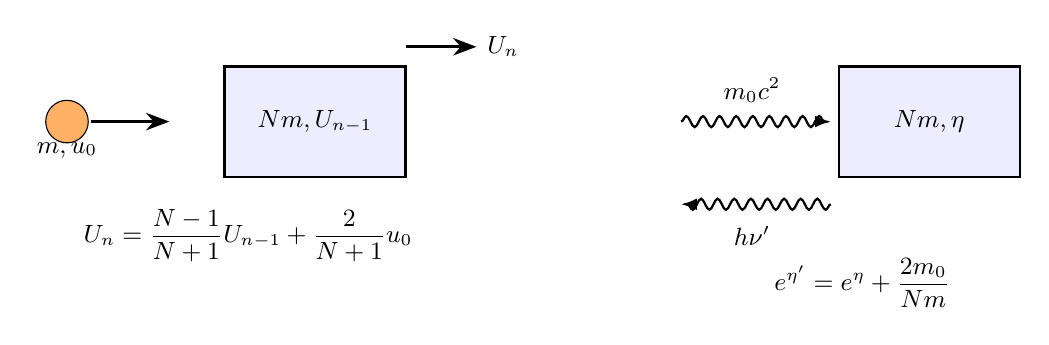
\begin{tikzpicture}[x=1cm,y=1cm,font=\small]

\begin{scope}[shift={(-3.8,0)}]
    \filldraw[fill=orange!60] (-2,0) circle (.27) node[below=4pt] {$m,u_0$};
    \draw[vec] (-1.7,0)--(-.7,0);
    \draw[body] (0,-.7) rectangle (2.3,.7); \node at (1.15,0) {$Nm,U_{n-1}$};
    \draw[vec] (2.3,.95)--(3.2,.95) node[right] {$U_n$};
    \node at (.3,-1.45) {$U_n=\dfrac{N-1}{N+1}U_{n-1}+\dfrac{2}{N+1}u_0$};
  \end{scope}
  \begin{scope}[shift={(4.3,0)}]
    \draw[body] (-.3,-.7) rectangle (2.0,.7); \node at (.85,0) {$Nm,\eta$};
    \draw[decorate,decoration={snake,amplitude=2pt,segment length=6pt},-{Latex[length=2mm]},thick] (-2.3,0)--(-.4,0);
    \draw[decorate,decoration={snake,amplitude=2pt,segment length=6pt},-{Latex[length=2mm]},thick] (-.4,-1.05)--(-2.3,-1.05);
    \node at (-1.4,.4) {$m_0c^2$}; \node at (-1.4,-1.45) {$h\nu'$};
    \node at (0,-2.05) {$e^{\eta'}=e^\eta+\dfrac{2m_0}{Nm}$};
  \end{scope}

\end{tikzpicture}

% 15 question-08
\begin{tikzpicture}[x=1cm,y=1cm,font=\small]

\draw[thick](-.7,0)--(7,0) (-.7,3)--(3,3);\draw[thick](3,3)--(3.9,3) (4.1,3)--(5,3);\draw[thick](3.9,2.68)--(3.9,3.32) (4.1,2.68)--(4.1,3.32);\node[above]at(4.0,3.33){$C,\lambda U_0$};\draw[thick](5,3)--(7,3);
\draw[very thick,blue](0,0)--(0,3);\node[left]at(0,1.5){杆 $m,L$};\draw[velocity](.4,1.5)--(1.6,1.5)node[right]{$v$};
\draw[thick](5.8,3)--(5.8,1.8) (5.8,1.3)--(5.8,0);\draw[body](5.55,1.8)--(6.05,1.8)--(5.8,1.3)--cycle;\draw[thick](5.5,1.3)--(6.1,1.3);
\draw[thick](6.7,3)--(6.7,1.7) (6.7,1.2)--(6.7,0);\draw[body](6.45,1.2)--(6.95,1.2)--(6.7,1.7)--cycle;\draw[thick](6.4,1.7)--(7,1.7);
\node[above]at(6.3,3.25){反并联二极管};\node[right]at(7.2,1.5){阈值 $U_0$};
\draw[dim](2.3,0)--(2.3,3)node[midway,right]{$l$};\node at(3.2,1.8){$\otimes B$};\node at(3.2,-.6){电容串入上导轨；二极管两端接上下导轨};

\end{tikzpicture}

% 16 solution-08
\begin{tikzpicture}[x=1cm,y=1cm,font=\small]

\begin{scope}[shift={(-3.8,0)}]
    \draw[->] (-.5,0)--(7.1,0) node[right] {$\lambda$};
    \draw[->] (0,-2.1)--(0,2.1) node[above] {$F(\lambda)=y_f/U_0$};
    \draw[very thick,blue!70!black] (0,0)--(1,1)--(3,-1)--(5,1)--(7,-1);
    \foreach \x in {1,3,5,7}{\draw (\x,.1)--(\x,-.1) node[below=3pt] {$\x$};}
    \draw[guide] (-.3,1)--(7,1) (-.3,-1)--(7,-1);
    \node at (3.4,-2.6) {$F(\lambda+4)=F(\lambda)$};
  \end{scope}
  \begin{scope}[shift={(5.0,0)}]
    \draw[body] (-2,-.6) rectangle (2,.6); \node at (0,0) {等效 $LC'$ 振荡器};
    \draw[current] (-2.5,1.2)--(1.8,1.2) node[midway,above] {$i$};
    \node at (0,-1.35) {$\dfrac1{C'}=\dfrac1C+\dfrac{B^2l^2}{m}$};
    \node at (0,-2.15) {$v_\infty=\dfrac{BlC'U_0}{m}[\lambda-F(\lambda)]$};
  \end{scope}

\node[align=center]at(5,-3.0){二极管耗能 $U_0|i|$\\$F$ 周期，末速 $v_f$ 非周期};
\end{tikzpicture}

\end{document}
